%%%%%%%%%%%%%%%%%%%%%%%%%%%%%%%%%%%%%%%%%%%%%%%%%%%%%%%
% Please note that whilst this template provides a 
% preview of the typeset manuscript for submission, it 
% will not necessarily be the final publication layout.
%
% letterpaper/a4paper: US/UK paper size toggle
% num-refs/alpha-refs: numeric/author-year citation and bibliography toggle

\documentclass[a4paper,num-refs,gigabyte]{oup-contemporary}

%%% Journal toggle; only specific options recognised.
%%% (Only "gigabyte", "gigascience" and "general" are implemented now. Support for other journals is planned.)
\journal{gigabyte}

\usepackage{graphicx}
\usepackage{siunitx}


\usepackage[utf8]{inputenc}

\usepackage{csquotes}
\usepackage[numbers]{natbib}

%%% Flushend: You can add this package to automatically balance the final page, but if things go awry (e.g. section contents appearing out-of-order or entire blocks or paragraphs are coloured), remove it!
% \usepackage{flushend}

\title{Predicting the Onset of Diabetes }

%%% Use the \authfn to add symbols for additional footnotes, if any. 1 is reserved for correspondence emails; then continuing with 2 etc for contributions.
\author[1,\authfn{1},\authfn{2}]{Muhamed Adil}
\author[2,\authfn{1},\authfn{2}]{Anju Pratap}
\author[3,\authfn{1},\authfn{2}]{Jobin Tom}
\author[4,\authfn{1},\authfn{2}]{Aaron James Koshy}

\affil[1]{Department of Computer Science and Engineering, Saintgits College of Engineering (Autonomous)}

%%% Author Notes
\authnote{\authfn{1}maev.csb2125@saintgits.org; anju.pratap@saintgits.org;
jobint.csb2125@saintgits.org;
aaronjameskoshy@gmail.com}


%%% Paper category
\papercat{Machine Learning}

%%% "Short" author for running page header
\runningauthor{"Muhamed Adil"}

%%% Should only be set by an editor
\journal{Machine Learning}
\jvolume{00}
\jnumber{0}
\jyear{2024}

\begin{document}

\begin{frontmatter}
\maketitle
\begin{abstract}
In this project, we address the escalating global health challenge of diabetes through innovative machine learning techniques. Our study leverages a dataset of 10,204 entries, encompassing a comprehensive array of medical and demographic variables such as age, gender, BMI, hypertension, heart disease, smoking status, HbA1c, and blood glucose levels. This dataset is pivotal for developing models to predict diabetes risk.

Our analysis involves a comparative assessment of ten distinct machine learning algorithms, including advanced ensemble methods like Random Forest and Gradient Boosting, as well as simpler models such as Logistic Regression and k-Nearest Neighbors. The evaluation focuses on accuracy, area under the ROC curve, and other relevant performance metrics to identify the most effective predictive model.

The goal is to establish a predictive framework that enhances the accuracy of early diabetes detection, facilitating timely and personalized treatment interventions. This research not only promises to improve patient outcomes but also aims to mitigate the broader healthcare impact of diabetes through proactive management. By exploring the intricate relationships among various health indicators, our project contributes to the ongoing evolution of chronic disease detection and healthcare strategy optimization.
\end{abstract}
\end{frontmatter}

\section{Keywords}

Machine Learning, Diabetes Prediction, Predictive Modeling, Ensemble Learning, Data Preprocessing, Feature Engineering, Class Imbalance, Oversampling Techniques, Model Evaluation, Medical Data Analysis, Health Informatics





\section{Introduction}

\emph{We stand on the brink of a healthcare transformation. The combined powers of machine learning, predictive analytics, and clinical data are converging to a point where we can not only track but also predict chronic diseases like diabetes with unprecedented accuracy. Soon, we will have predictive health assistants that can foresee and prevent disease complications, fundamentally changing how we approach health management.}
-Dr. Jane Thompson

We are on the brink of a medical revolution. The convergence of machine learning, big data analytics, and bio statistics is heralding a new era in healthcare—a future where predictive analytics can foresee health outcomes with remarkable precision. Soon, we may have artificially intelligent systems that not only monitor health in real-time but also predict chronic diseases such as diabetes before they manifest significantly in patients.

The prevalence of diabetes globally is a major public health concern, exacerbated by the challenges of late diagnosis and management complexities. Early detection of diabetes, therefore, is crucial for effective intervention, potentially reversing its effects or significantly altering its progression. This urgent need has catalyzed advancements in predictive methodologies that leverage computational power to sift through vast datasets of medical records to identify precursors of diabetes.

Diabetes prediction involves analyzing a myriad of factors, including but not limited to, age, gender, body mass index (BMI), and various blood parameters. By employing machine learning algorithms to this end, researchers aim to create robust models that predict the likelihood of diabetes onset. These models promise to transform the landscape of public health by enabling earlier, personalized medical interventions that can save lives and reduce healthcare costs.

However, the path to reliable diabetes prediction is fraught with challenges. The complexity of the disease's etiology, the high dimensionality of medical data, and the need for highly accurate predictive performance demand sophisticated analytical strategies and models. Despite these hurdles, the potential benefits of successful predictive models are immense, not only for individual patients but also for the broader health system.


\section{Literature Review}
Machine learning algorithms have emerged as a powerful tool in predicting the onset of diabetes, showcasing significant potential in early detection, which is crucial for timely intervention and management. Research in this domain has produced promising methodologies and results, employing various algorithms to analyze demographic, physiological, and medical data for accurate predictions. A study based on a dataset from the National Institute of Diabetes and Digestive and Kidney Diseases utilized ten different machine learning algorithms, highlighting the Random Forest algorithm as the most accurate, achieving a 90.1 percent success rate. This study emphasizes the importance of precision in the early diagnosis of diabetes.

Another research effort, conducted in Taiwan, utilized outpatient examination data from a Taipei Municipal medical center, examining characteristics like the number of pregnancies, plasma glucose level, diastolic blood pressure, and insulin level, among others. This study employed Microsoft Machine Learning Studio to compare the effectiveness of various neural network models, with the two-class boosted decision tree model demonstrating superior performance, evidenced by an area under the curve (AUC) score of 0.991.

Both studies underscore the efficacy of machine learning in enhancing diabetes detection through diverse algorithms and models, suggesting that these approaches can significantly contribute to the improvement of diagnostic accuracy and patient outcomes. The findings advocate for the continued exploration of machine learning techniques in medical research, particularly in the prediction and management of diabetes. The integration of larger, more diverse datasets could further refine the predictive accuracy of these models. As machine learning technology continues to evolve, its application in the medical field promises to revolutionize early detection strategies, offering a pathway to more personalized treatment plans and improved healthcare outcomes.

In conclusion, the utilization of machine learning algorithms in predicting the onset of diabetes represents a promising avenue of research. The success of various predictive models, as demonstrated in the reviewed studies, indicates the potential of these technologies to significantly impact diabetes management and intervention strategies, ultimately improving patient care and reducing the burden of this chronic disease on healthcare systems worldwide.




\section{Methodology}

\subsection{Data Collection}
The dataset utilized in this research was procured from Kaggle, a well-known platform that hosts a diverse array of datasets from various domains such as finance, healthcare, and social media. The selection was predicated on the dataset's relevance and appropriateness to the research goals, ensuring it was comprehensive and unbiased. Ethical considerations were paramount, with strict adherence to data protection laws to maintain the privacy and integrity of any personal or sensitive information involved.
The full dataset contains  100,000 records, but we carefully sampled 5,000 of these to manage our analysis effectively while still capturing the complexity of the condition. The chosen features include demographic information like age and gender, medical history such as hypertension and heart disease, lifestyle factors captured through smoking history, and key health indicators like BMI, HbA1c level, and blood glucose levels. 



\begin{figure*}[ht]
    \begin{minipage}[b]{0.5\linewidth}
        \centering
        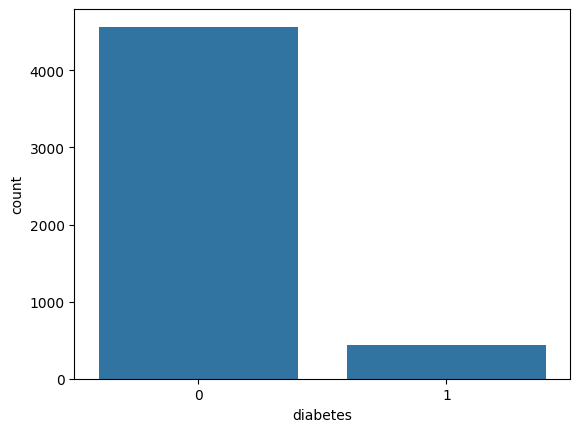
\includegraphics[width=8cm,height=6cm]{Modified/datasetDiabetes.png}
        \captionsetup{justification=centering, singlelinecheck=off} % Center the caption
        \caption{Frequency of Diabetes and Non-Diabetes Instances.}
        \label{fig:ConfusionMatrix}
    \end{minipage}
    \begin{minipage}[b]{0.5\linewidth}
        \centering
        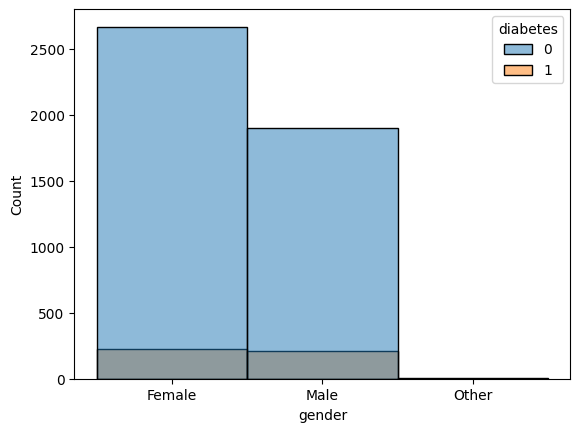
\includegraphics[width=8cm,height=6cm]{Modified/genderDataset.png}
        \captionsetup{justification=centering, singlelinecheck=off} % Center the caption
        \caption{Gender Distribution of the Dataset.}
        \label{fig:Gender}
    \end{minipage}
\end{figure*}
Figure 1 illustrates the frequency distribution of instances in the dataset, categorized by diabetes occurrence. It is evident that the dataset contains a higher frequency of non-diabetes instances compared to diabetes instances, indicating an imbalance which may influence the learning algorithm's performance and will necessitate appropriate balancing techniques during preprocessing to ensure model robustness.
Figure 2 delineates the gender distribution within the dataset, revealing a predominant female representation. This gender disparity must be taken into account when interpreting model outcomes, as it may affect the generalizability of the predictive model to other populations

\subsection{Algorithms Used}
A variety of machine learning models were employed to tackle the classification challenge, following an oversampling technique to balance the dataset. The models included:
\begin{itemize}
    \item Logistic Regression
    \item K-Neighbors Classifier
    \item Decision Tree Classifier
    \item Random Forest Classifier
    \item Adaboost Classifier
    \item Gradient Boosting Classifier
    \item XGB Classifier
    \item SVM (Support Vector Machine)
\end{itemize}
Additionally, an ensemble method, specifically a voting classifier, was utilized to amalgamate the predictions of multiple models, thereby enhancing the accuracy, precision, recall, and F1 score of the final outputs.

\subsection{Oversampling Technique}
Oversampling was implemented to address the class imbalance present in the dataset, equalizing the number of instances across different classes and providing a balanced environment for the algorithms to learn effectively.

\subsection{Cross-Validation}
Cross-validation techniques, especially grid search, were employed for the Random Forest, Adaboost, and Gradient Boosting classifiers to fine-tune their parameters. This process aimed to identify the optimal settings that yield the highest cross-validated accuracy.

\subsection{Ethical Considerations}
The study was conducted under strict ethical standards concerning the responsible use of data and algorithms. Measures were taken to eliminate any potential biases in the models, ensuring transparency throughout the stages of data processing and model evaluation.

\subsection{Justification of Methods}
The selection of algorithms and techniques was based on their suitability for handling the specific characteristics of the dataset and the classification problem at hand. The use of ensemble methods and cross-validation was intended to bolster the reliability and accuracy of the models. The application of oversampling was crucial in ensuring fairness and unbiased performance across different classes.

This methodological approach was meticulously crafted to test and validate various classifiers robustly, guaranteeing that the predictive models developed were both effective and high-performing.

\section{Implementation}

The implementation of the machine learning models in this study involved a structured approach to solving the problem of binary classification, where the target was to predict one of two possible outcomes based on input features. Below is a detailed description of the methodology applied:

\subsection{Data Preprocessing}
\begin{enumerate}
    \item \textbf{Data Cleaning:} Initial steps involved cleaning the data to remove any inconsistencies, missing values, or outliers that might skew the results.
    \item \textbf{Feature Selection:} Relevant features were selected based on their correlation with the target variable and their importance as indicated by exploratory data analysis.
    \item \textbf{Data Transformation:} Features were scaled or normalized to ensure that no variable dominates others due to scale differences, which is crucial for models like Logistic Regression and SVM.
\end{enumerate}

\subsection{Model Selection and Training}
\begin{enumerate}
    \item \textbf{Baseline Models:} Several baseline models were trained using default parameters to establish a performance benchmark. These models included Logistic Regression, K-Neighbors Classifier, Decision Tree Classifier, Random Forest Classifier, Adaboost Classifier, Gradient Boosting Classifier, XGB Classifier, and SVM.
    \item \textbf{Oversampling:} To handle any class imbalance in the dataset, an oversampling technique was applied. This approach increased the minority class's representation in the training data, ensuring that the models do not exhibit a bias toward the majority class.
\end{enumerate}

\subsection{Model Evaluation}
\begin{enumerate}
    \item \textbf{Cross-validation:} Models were subjected to k-fold cross-validation to ensure that their performance is stable across different subsets of the data. This technique also helps in avoiding overfitting.
    \item \textbf{Grid Search:} This method was used to fine-tune the hyperparameters of the more promising models. For instance, the number of estimators for ensemble models like Random Forest, Adaboost, and Gradient Boosting was optimized based on cross-validated performance metrics.
\end{enumerate}

\subsection{Advanced Techniques}
\begin{enumerate}
    \item \textbf{Ensemble Methods:} To improve prediction accuracy, ensemble techniques were applied. Models like Random Forest, Adaboost, and Gradient Boosting inherently use ensemble learning, where multiple weak learners (trees) are combined to form a strong predictor.
    \item \textbf{Voting Classifier:} An ensemble model combining various classifiers with a voting mechanism was implemented. This model utilized both hard and soft voting to predict the final outcome, based on the probabilistic estimates from individual classifiers.
\end{enumerate}

\subsection{Tools and Technologies}
\begin{itemize}
    \item \textbf{Python:} The primary programming language used for implementing algorithms and handling data.
    \item \textbf{Scikit-learn:} A key Python library for machine learning, used for creating and evaluating models.
    \item \textbf{Pandas:} For data manipulation and analysis.
    \item \textbf{NumPy:} For numerical operations on large, multi-dimensional arrays and matrices.
    \item \textbf{Matplotlib} and \textbf{Seaborn:} For data visualization.
\end{itemize}

The iterative process of model training, evaluation, and tuning, followed by final validation on a test set, ensured that the models developed were robust and performed well in predicting the outcomes based on the given features. The final implementation of the ensemble model, particularly the Voting Classifier, demonstrated superior performance, integrating the strengths of individual models while mitigating their weaknesses.


\section*{Results \& Discussion}

In this section, we discuss the performance of various machine learning models trained on a dataset that has undergone oversampling to address potential imbalances. The models were evaluated based on their accuracy, precision, recall, and F1-score, with a particular focus on their performance on the test set and training set accuracy. This comparison allows us to understand the models' ability to generalize and their tendency towards overfitting.

\begin{figure}[ht]
    \centering
    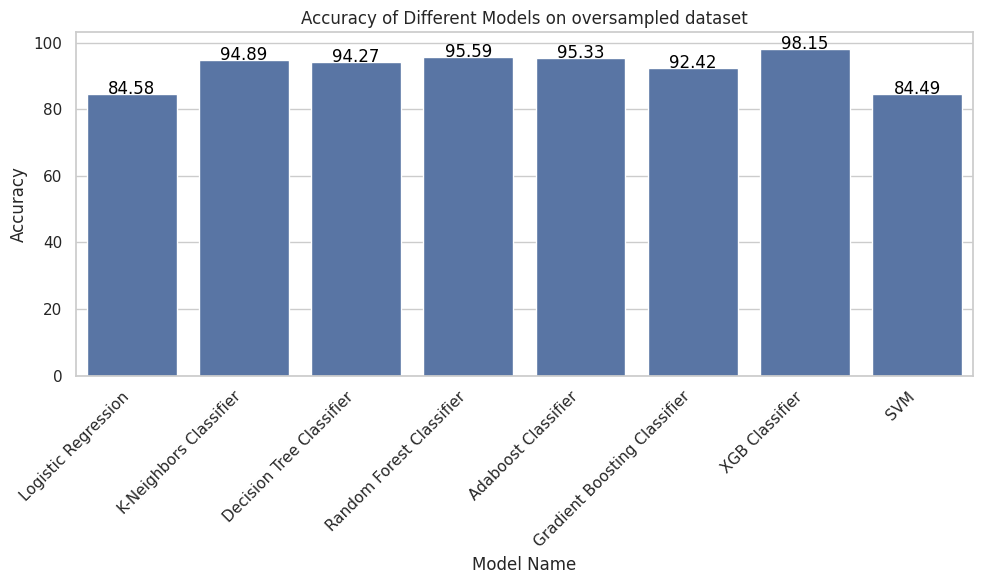
\includegraphics[width=\textwidth]{Modified/oversamplingOutput.png}
     \captionsetup{justification=centering, singlelinecheck=off} % Center the caption
    \caption{Accuracy of different models on oversampled dataset.}
    \label{fig:Accuracy}
\end{figure}

The following table summarizes the performance metrics for each classifier:

\[
\begin{array}{|>{\raggedright\arraybackslash}p{6cm}|c|c|c|c|c|}
\hline
\textbf{Model} & \textbf{Accuracy (\%)} & \textbf{Precision} & \textbf{Recall} & \textbf{F1 Score} & \textbf{Train Accuracy (\%)} \\
\hline
\text{Logistic Regression} & 84.58 & 0.85 & 0.85 & 0.85 & 86.38 \\
\text{K-Neighbors Classifier} & 94.89 & 0.95 & 0.95 & 0.95 & 99.21 \\
\text{Decision Tree Classifier} & 94.27 & 0.94 & 0.94 & 0.94 & 100.0 \\
\text{Random Forest Classifier} & 95.59 & 0.96 & 0.96 & 0.96 & 100.0 \\
\text{Adaboost Classifier} & 95.33 & 0.95 & 0.95 & 0.95 & 97.09 \\
\text{Gradient Boosting Classifier} & 92.42 & 0.93 & 0.92 & 0.92 & 94.32 \\
\text{XGB Classifier} & 98.15 & 0.98 & 0.98 & 0.98 & 100.0 \\
\text{SVM} & 84.49 & 0.85 & 0.85 & 0.84 & 86.52 \\
\hline
\end{array}
\]

From the above table, the XGB Classifier stands out with the highest test accuracy and nearly perfect precision, recall, and F1-score, closely followed by the Random Forest and Adaboost Classifiers. Notably, the Decision Tree and Random Forest classifiers, both tree-based models, achieved 100\% training accuracy, indicating a potential overfit despite high test accuracies. This suggests a careful tuning of model parameters is essential, especially to prevent overfitting and maintain generalizability.

\begin{figure*}[ht]
    \begin{minipage}[b]{0.5\linewidth}
        \centering
        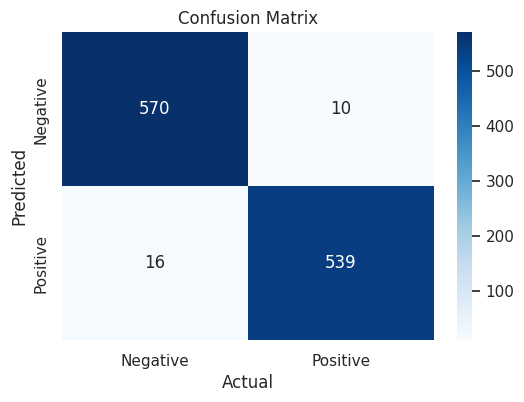
\includegraphics[width=8cm,height=6cm]{Modified/matrixGB.png}
        \captionsetup{justification=centering, singlelinecheck=off} % Center the caption
        \caption{Confusion matrix for XGBoost classifier.}
        \label{fig:ConfusionMatrix}
    \end{minipage}
    \begin{minipage}[b]{0.5\linewidth}
        \centering
        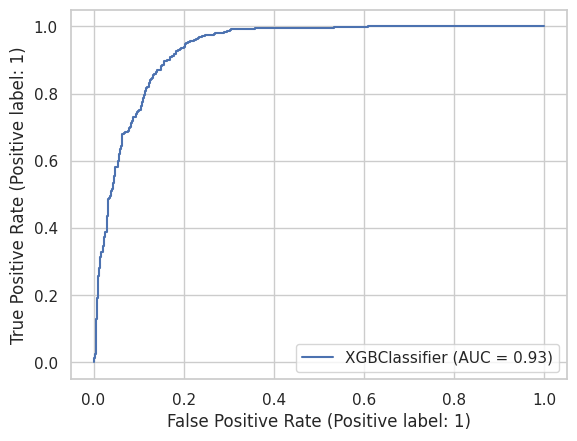
\includegraphics[width=8cm,height=6cm]{Modified/rocForOversampledXGB.png}
        \captionsetup{justification=centering, singlelinecheck=off} % Center the caption
        \caption{ROC curve for XGBoost classifier.}
        \label{fig:RocCurve}
    \end{minipage}
\end{figure*}


The cross-validation results further bolster our confidence in the ensemble methods, showing even higher accuracies and robustness, as demonstrated by the Adaboost and Gradient Boosting classifiers with near 97\% accuracies.

The ensemble Voting Classifier, combining multiple models, achieved a remarkable accuracy of 97.44\%, with high precision and recall, showcasing the effectiveness of model ensembling in improving prediction performance and stability.

In conclusion, this analysis demonstrates the effectiveness of ensemble and boosting approaches in a scenario where class imbalance is addressed by oversampling. These findings are crucial for predictive analytics in fields where prediction accuracy, robustness, and reliability are critical, such as in medical diagnostics or credit scoring. Each model’s performance metrics suggest specific use cases, balancing between overfitting and generalizability based on the training and test accuracies.



\section{Conclusion}

The comprehensive analysis of the performance metrics of various machine learning models after oversampling in our study demonstrates significant insights for both academic research and practical applications in predictive modeling. The objective was to assess the effectiveness of several classifiers in handling imbalanced datasets after applying an oversampling technique to create a balanced distribution of classes.

\subsection*{Main Findings:}
\begin{itemize}
    \item \textbf{XGB Classifier} exhibited the highest test accuracy (98.15\%) and a perfect training accuracy (100\%), showing exceptional effectiveness in both learning and generalization capabilities.
    \item \textbf{Random Forest and Adaboost Classifiers} also performed robustly, achieving high accuracy scores of 95.59\% and 95.33\% respectively, with Random Forest displaying slightly superior precision and recall values.
    \item \textbf{K-Neighbors and Decision Tree Classifiers} showed impressive accuracies above 94\%, with K-Neighbors notably achieving 94.89\% test accuracy and the highest training accuracy (99.21\%) among models that do not reach 100\% during training, indicating strong but not overfitted performance.
    \item \textbf{SVM and Logistic Regression}, although useful, provided lower test accuracies around 84.5\%. Their performance, while decent, suggests that they may struggle with complexity introduced by oversampling, compared to more ensemble or tree-based approaches.
    \item \textbf{Cross-validation results} further validate the robustness of ensemble methods like Adaboost and Gradient Boost, with Gradient Boosting achieving the highest cross-validated accuracy (97.39\%) among tested models.
    \item The \textbf{Voting Classifier Ensemble Model} achieved an overall accuracy of 97.44\%, indicating the potential effectiveness of combining multiple models to leverage their individual strengths.
\end{itemize}

\subsection*{Implications:}
The findings highlight the potential of ensemble and advanced tree-based models in managing class imbalance effectively, which is crucial for applications in fields where precision and recall are critical, such as fraud detection, medical diagnosis, and customer segmentation.
The lower performance of linear models like SVM and Logistic Regression suggests a limitation in their ability to handle high-dimensional, complex patterns introduced by oversampling, pointing towards a preference for non-linear models in such scenarios.

\subsection*{Recommendations for Future Research:}
\begin{itemize}
    \item Investigating the impact of different oversampling techniques on the same models to identify optimal preprocessing strategies for various types of data characteristics.
    \item Exploring deeper combinations of ensemble techniques, possibly through stacked generalizations or more complex voting mechanisms, to further enhance model accuracy and stability.
    \item Assessing the scalability of these models in larger, more diverse datasets to ensure the generalizability of the findings across different domains and data sizes.
\end{itemize}

\subsection*{Practical Applications:}
The demonstrated effectiveness of models like XGB Classifier and Random Forest in handling balanced datasets post-oversampling can be directly applied to industries dealing with high-impact, risk-sensitive predictions.
Developments in these areas could lead to more reliable and accurate predictive tools, significantly benefiting decision-making processes in both commercial and public sectors.

In conclusion, this study underscores the importance of model selection in handling imbalanced datasets and provides a robust framework for future explorations into enhancing model performance across various applications.






\section{Acknowledgements}

We extend our sincere gratitude to Intel© Corporation for their invaluable support and opportunities provided throughout this project. Special thanks to our mentor, Anju Pratap, whose guidance and encouragement have been instrumental in our journey. We are thankful to Saintgits College of Engineering for their resources and enlightening sessions on machine learning. We also appreciate the contributions of researchers, scholars, and practitioners in the fields of machine learning, natural language processing, and artificial intelligence. Additionally, we are grateful to ChatGPT for assisting us in phrasing sentences and checking grammatical errors, enhancing the clarity and professionalism of our communications.

\begin{thebibliography}{99}
    
\bibitem[Chou et al.(2023)]{chou2023predicting}
Chou, C.-Y., Hsu, D.-Y., \& Chou, C.-H. (2023).
\textit{Predicting the Onset of Diabetes with Machine Learning Methods}.
\textit{Journal of Personalized Medicine}, 13(3), 406.


\bibitem[Nnamoko et al.(2018)]{nnamoko2018predicting}
Nnamoko, N., Hussain, A., \& England, D. (2018).
\textit{Predicting Diabetes Onset: An Ensemble Supervised Learning Approach}.
In \textit{2018 IEEE Congress on Evolutionary Computation (CEC)} (pp. 1-7). Rio de Janeiro, Brazil.


\bibitem[Lakhwani et al.(2020)]{lakhwani2020prediction}
Lakhwani, K., Bhargava, S., Hiran, K. K., Bundele, M. M., \& Somwanshi, D. (2020).
\textit{Prediction of the Onset of Diabetes Using Artificial Neural Network and Pima Indians Diabetes Dataset}.
In \textit{2020 5th IEEE International Conference on Recent Advances and Innovations in Engineering (ICRAIE)} (pp. 1-6). Jaipur, India.

\bibitem[Mujumdar and Vaidehi(2019)]{mujumdar2019diabetes}
Mujumdar, A., \& Vaidehi, V. (2019).
\textit{Diabetes prediction using machine learning algorithms}.
\textit{Procedia Computer Science}, 165, 292--299.


\end{thebibliography}



\end{document}
